\chapter{BACKGROUND}
\label{background}

\section{Graphs}
A graph $G = (V, \varepsilon)$ is defined by a set of nodes $V$ and a set of edges $E$ between these nodes as going from node $u \in V$ to node $v \in V$ as $(u,v) \in \varepsilon$. In this thesis, we concern only simple graphs, i.e., there exists at most one edge between each pair of nodes, and no edges between  a node and itself. Moreover, all edges are undirected, so $(u,v) \in \varepsilon \longleftrightarrow (u,v) \in \varepsilon$. A graph has a single type of edge or different type of edges. In a multi-relational graph the edge notation can be extended as $(u,\tau,v) \in \varepsilon$ to include the relation type $\tau$ \cite{hamilton2020graph}. Throughout the thesis we consider two important subsets of graphs; homogeneous and heterogeneous i.e., graphs with single and multiple relation types respectively. 

Graph is homogeneous when all the nodes represents the instances of the same type and all the edges represents the same type of relations. For instance, drug-drug interaction network is a homogeneous graph consisting of drugs and the connections between drugs, representing the same type of entity. Figure \ref{fig:sample_ddi} shows a homogeneous drug-drug interaction graph with five drugs, and the risk or severity of bleeding can be increased when Cyclosporine is combined with Phenylalanine \cite{ihlefeldt2014polymorphs}. 

\begin{figure}
    \centering
        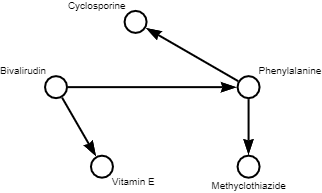
\includegraphics[width=0.5\linewidth]{chapters/background/figures/ddi.png} 
    \caption{Homogeneous Drug-Drug Interaction Graph.}
    \label{fig:sample_ddi}
\end{figure}

Graph is heterogeneous if the set of nodes can be partitioned into disjoint sets $V = V_{1} \cup V_{2} \cup ... \cup V_{k} $ where $V_{i} \cap V_{j} = \emptyset , \forall i \neq j$ \cite{sun2013mining}. For instance, drug-disease network is a heterogeneous graph consisting of two types of nodes as drugs and diseases, and two types of edges representing the \textit{treatment} relation that occurs only between drug nodes and disease nodes, and similarly \textit{polypharmacy side effect} that occurs only between two drug nodes. Figure \ref{fig:sample_ddi} shows a heterogeneous drug-disease association graph with 4 drugs, three disease, and two types of edges. For instance, the risk or severity of neutropenia can be increased when Methyclothiazide is combined with Phenylalanine \cite{ruiz2022primary}. 

\begin{figure}
    \centering
        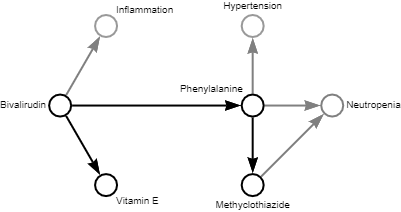
\includegraphics[width=0.65\linewidth]{chapters/background/figures/dda.png} 
    \caption{Heterogeneous Drug-Disease Association Graph.}
    \label{fig:sample_dda}
\end{figure}


\section{Graph Representation Learning}
The rapid development of molecular biology, bioinformatics, and cheminformatics and the increase in the number of available data have led the modeling the biological components as nodes and the interactions between nodes as edges of graphs. In the case of the drug discovery and disease treatment, it is crucial to examine the interactions between drug-drug, drug-disease, drug-protein, and protein-disease \cite{daminelli2012drug, davis2009comparative}. These interactions can be formed as heterogeneous graphs and used in knowledge extraction. Traditional machine learning algorithms use the data represented in Euclidean domain such as 1D sequences of proteins, 2D biomedical image, or 3D protein structure. However, graphs form a non-Euclidean domain and create a challenge due to its complex topological structure, diverse node connections, and arbitrary neighbor size. To address these challenges, graph representation learning is employed. Graph representation learning or graph embedding learns the low-dimensional representations of node or edges that can be used in downstream graph analytics or machine learning tasks such as node classification, and link prediction.

We use graph-based distributional representation learning method to represent the molecules. In general, this set of methods represents data that cannot be expressed in Euclidean space as a graph, and it aims to learn distributed vectors that reflect the semantic connections in the graph for nodes, edges or underlines in this graph \cite{wu2019comprehensive}. One of the most important advantages of this approach is that it can express the relationships between different types of nodes. Using the compiled data (See details in Chapter \ref{chapter:dataset_preparation}) we model protein, ligand, disease and side effect information and the extracted language-based information as different node types in a graph. The relationship between each node corresponds to different relationships such as protein-drug interaction and protein-protein interaction in our graph. By using the heterogeneous graph structure that we have obtained in this way, we learn the graph-based representation vectors for proteins and chemicals. In this heterogeneous graph, when distributional representations for chemicals and proteins are learned, the relationships of nodes with different concepts such as disease and side effects are also included in the representations. In this way, the output of the received vectors becomes richer in terms of information. 

To learn the distributional representation vectors we use MetaPath2Vec \cite{dong2017metapath2vec, pal2016deep}, which is a framework to learn representations of heterogeneous graphs. It is a neural network model that is designed to capture the rich semantics embedded in heterogeneous graphs by exploiting different types of relationships and meta-paths among nodes. To generate meaningful representations, it considers different semantics of relations, i.e., different meta-paths which are the sequence of node/edge types that denote relationships between node pairs.

MetaPath2Vec formalizes the representation learning problem in heterogeneous networks by leveraging the definitions in \cite{dong2017metapath2vec, sun2013pathselclus} as follows:

A heterogeneous network is a graph $G = (V, E, T)$ in which node $v$ is associated with edge $e$ with mapping functions $\phi(v) : V \to T_{V}$ and $\varphi(e) : E \to T_{E}$, respectively. The aim of heterogeneous network representation learning is to learn the d-dimensional representation $X \in R^{|V|\times d}, d \ll |V|$ , given a heterogeneous network $G$, that is able to capture the topological and semantic relations among them. Therefore, the resulting representation is low-dimensional matrix $X$, with the $v^{th}$  row corresponding to the representation of node $v$. Regardless of the node types in $V$, representations of each node are mapped into the same latent space. 

The word2vec model is proposed to learn the distributed representations of words within a corpus \cite{mikolov2013efficient, mikolov2013distributed}. Thereafter, DeepWalk \cite{perozzi2014deepwalk} and node2vec \cite{grover2016node2vec} models proposed, aiming to map the word-context concept of word2vec model into a network. DeepWalk and node2vec models use random walks to map the word-context concept and utilize the skip-gram model to learn the node representation in a homogeneous network. Their objective is to maximize the network probability \cite{mikolov2013distributed, perozzi2014deepwalk, grover2016node2vec}, that is:
\begin{equation}
    arg \max_{\theta} \prod_{v \in V}^{} \prod_{c \in N(V)}^{} p(c|v;\theta)
\end{equation}

where $N(v)$ denotes the node $v$'s neighborhood, in which $v$'s one-hop neighbors, and $p(c|v;\theta)$ defines the conditional probability of a context node $c$ given node $v$.

In the same way, metapath2vec introduces the heterogeneous skip-gram model for heterogeneous networks to model the heterogeneous neighborhood of a node. Therefore, metapath2vec aims to maximize the probability of having the heterogeneous context $N_{t}(v), t \in T_{V}$ given a node $v$:

\begin{equation}
    arg \max_{\theta} \sum_{v \in V}^{} \sum_{t \in T_{V} }^{} \sum_{c_{t} \in N_{t}(V)}^{} p(c_{t}|v;\theta)
\label{eq:context}
\end{equation}

where $N_{t}(v)$ denotes the node $v$'s neighborhood with the $t^{th}$ type of nodes. The $p(c_{t}|v;\theta)$ is a softmax function \cite{bengio2013representation, mikolov2013distributed}, that is:

\begin{equation}
    p(c_{t}|v;\theta) = \frac{e^{X_{c_{t}}}.X_{v}}{\sum_{u \in V}^{} e^{X_{u}}.X_{v}}
\label{eq:softmax}
\end{equation}

where $X_{v}$ is the $v^{th}$ row of $X$, corresponding to the embedding vector for node $v$. Mikolov \textit{et al.} also introduce negative sampling \cite{mikolov2013distributed} for optimization. With negative sampling, a small set of words are sampled from the corpus to construct the softmax. Same technique is also applied for metapath2vec, and Equation \ref{eq:context} is updated as follows:

\begin{equation}
    log\sigma(X_{c_{t}}.X_{v}) + \sum_{m=1}^{M} \mathbb{E}_{u^{m}\sim P(u)}[log\sigma(-X_{u^{m}}.X_{v})]
\end{equation}

where $M$ is the negative sample size, $\sigma (x) = \frac{1}{1+e^{-x}}$ and $P(u)$ is the pre-defined distribution in which node $u^{m}$ is drew from $M$ times.

In order to transform heterogeneous network structures into metapath2vec's skip-gram, that design a meta-path-based random walks, and generate paths. A meta-path schema is a path, denoted as $V_{1} \xrightarrow[]{R_{1}} V_{2} \xrightarrow[]{R_{2}}\cdots V_{t} \xrightarrow[]{R_{t}} V_{t+1} \cdots \xrightarrow[]{R_{l-1}} V_{l}$, where $R = R_{1} \circ R_{2} \circ \cdots \circ R_{l-1}$ defines the composite relations between node types $V_{1}$ and $V_{l}$ \cite{sun2012mining}.

As shown above, metapath2vec uses random walks guided by meta-paths to generate heterogeneous node sequences that are rich in semantics and structural information, then it designs a heterogeneous skip-gram model to preserve the node $v$'s proximity to its neighborhood nodes. It uses Equation \ref{eq:softmax} to calculate the similarity a node and its neighbors.

Based on metapath2vec, several variants have been proposed. For instance, BHIN2vec \cite{lee2019bhin2vec} proposes an extension to the skip-gram technique in order to balance the influence different relation types on node embeddings. HHNE \cite{wang2019hyperbolic} performs random walks in hyperbolic spaces. Another method, Hin2vec \cite{fu2017hin2vec}, combines first-order and high-order relations to capture the heterogeneity of graph and carries out multiple relation prediction tasks to jointly learn the node embeddings. In this thesis we employ metapath2vec since it is simpler and convenient to apply to large heterogeneous graph. Moreover, its code is open, so it is freely available to use and easy to adapt.\footnote{Code available at: https://github.com/apple2373/metapath2vec}

\section{Language-Based Representation Vector Learning}

\section{Affinity Prediction}

\section{Evaluation}